% Este documento contiene el índice del manuscrito de la tesis.
%\documentclass[12pt,a4paper]{report}
%\usepackage{graphicx}
 
%\title{Introduction}
%\author{Claudia Guti\'errez}
%\date{ January 2018}


%\begin{document}

%\maketitle

%\tableofcontents{}

%%%%%%%%%%%%%%%%%%%%%%%%%%%%%%%%%%%%%%%%%%%%%%%%%%%%%%%%%%%%%%%%%%%%%%%%%%%%%%%%%%%%%%
\part{Introduction\label{cha:intro}}

%\section{Transversalidad}

% La ciencia aplicada o aplicación de la ciencia, ha evolucionado las sociedades a través de la conexión de los estudios de ciencia básica con los ingenios que implementaban el conocimiento estructural al día a día de los individuos. La construcción del puente entre los estudios fundamentales y su adaptación/evolución para el desarrollo de las sociedades, ha sido cuestión de una interpretación (y por lo tanto de intérpretes) capaz de econtrar el lenguaje adecuado para intercambiar este conocimiento.

%% Applied science has made societies evolved trough the linked between the basic science and the 'ingenios' that implement the structural knowdlege to the individual daylyligde. The bridge between the fundamental studies and its evolution or transformation into something applied for the societies development, has to be with the interpretation (so interpreters) that have been able to find the accurate languafe to exchange this knowdlege. %%

 % Esta transversalidad entre las disciplinas básicas de la física, la química o la biología con distintas acepciones prácticas, la mayoría de ellas recogidas bajo el paraguas de las ingenierías, desemboca ineludiblemente en una transformación de lo abstracto en lo tangible con la premisa o el ideal de mejorar el bienestar de las sociedades presentes y futuras. 

% Es sin embargo muy probable, que esta concepción de la aplicación científica haya desembocado en el mayor problema al que hacer frente desde.Siendo este antropocentrismo parte del problema, y no de la solución. Jorge Wasenberg escibe en su libro, ``el pensador intruso'' en referencia a la evolución de la ciencia y el progreso subyacente lo siguiente:

% ``Existen sobre todo dos vicios que tienden a inyectar ideología precocinada en la ciencia. Una de ellas se basa en las distintas formas de antropocentrismo y consiste en situar instintivamente al sujeto del conocimiento en el centro del cosmos. La historia del conocimiento es testigo: cada vez que barremos el Yo del centro del escenario el conocimiento avanza, y avanza sólo por ello.''

% Sin caer en lo pretencioso, este trabajo contribuye a la imbricación entre la ciencia del cambio climático y la tecnología renovable de producción eléctrica con mayor potencial a día de hoy, la solar fotovoltaica.

\chapter{Context and introduction\label{context}}

\epigraphfontsize{\small\itshape}
\epigraph{''Begin at the beginning,'' the King said gravely, ''and go on till you
come to the end: then stop.''}{--- \textup{Lewis Carroll}, Alice in Wonderland}

\section{A changing world} 

% Ideas a desarrollar:

% * Un mundo en constante evolución.
% * Cambio climático
% * Transición energética global
% * Cambios sociales/políticos.
% * Migraciones

%Se dice que nada es permanente excepto el cambio. Nos encontramos en un mundo en constante evolución donde inevitablemente algunos de los cambios que nos acontecen nos sobrepasarán sin que seamos capaces de adaptarnos a ellos. Mientras, otros pasarán desapercibidos a nuestros ojos por su lentitud o por no encontrarse en el centro de nuestras preocupaciones. Resulta paradójico pensar que algunos de esos cambios provocados por el ser humano, consciente o incoscientemente, con voluntad o por equivocación, obligarán al mismo como espcecie a resistir y adaptarse frente a las consecuencias de aquello que ellos mismos generaron. 

It is said that nothing is permanent except for change. We are in a constantly evolving world where, unavoidably, some of these changes will go over us without us  being able to adapt to them. Meanwhile, other changes will go unnoticed because of their slowness or because they are not part of our main concerns. It seems paradox to think that some of those human induced changes, consciously or unconsciously, willingly or by mistake, will make human beings resist an get adapted as a species against the consequences of something that they themselves created. 

%El desarrollo y la evolución de los pueblos ha estado ligado desde la primera Revolución Industrial a un incremento en la demanda de energía. El uso de los combustibles fósiles desde la invención de la máquina de vapor ha cambiado la forma de vida de las sociedades. Asociadas a este crecimiento, las emisiones de gases de efecto invernadero y su concentración en la atmósfera se han disparado con respecto a la época pre-Industrial [ref]. El calentamiento global, con su origen en las actividades humanas, supone uno de los mayores retos de adaptación para el ser humano. El carácter anisotrópico de los impactos asociados al cambio climático pone a prueba la solidaridad con las comunidades más vulnerables y menos responsables en este dilema.[ref]

The evolution and development of nations has been linked since the first Industrial Revolution to an increment on the energy demand. The use of fossil fuels since the vapor engine has changed the wellbeing of societies. Related to this increase, the green house gasses (GHG) emissions and their concentration in the atmosphere has risen dramatically in contrast to pre-Industrial times. Global warming, with its origin in human activities, is one of the biggest challenges of adaptation for human beings. The \textit{anisotropic} character of the associated impacts of climate change puts our solidarity with the most vulnerable and less responsible communities on trial.

%Para algunos estamos sumergidos en lo que ha sido descrito como una Tercera Revolución Industrial (ref), un proceso de desarrollo científico-tecnológico exponencial, donde convergen el desarrollo de las tecnologías renovables con el uso masivo de las nuevas tecnologías de la comunicación. La transición energética en marcha debería ser la respuesta a una demanda de una ciudadanía comprometida que encuentra en estas tecnologías una alternativa y una respuesta a los problemas medioambientales y sus consecuencias asociadas. 

Some people believe we are in what has been described as the Third Industrial Revolution (ref), a process of exponential scientific-technological development, characterized as a convergence of the evolution of renewable energy technologies and the massive use of new communication technologies. The ongoing energy transition should be the answer to committed citizens that find those technologies as an alternative and an answer to the environmental challenges and associated consequences.     

%El contexto actual está caracterizado por una avanzada globalización donde se han difuminado las fronteras gracias al desarrollo de las telecomunicaciones y los movimientos migratorios internacionales son más factibles [ref]. En 2015, había 100 millons más de personas residiendo en un país diferente al de su nacimiento que en 1990 [International Organization for Migration]. La mayoría de éstos movimientos están relacionados con oportunidades laborales o cuestiones familiares. Sin embargo, el crecimiento de la población y el aumento indefinido de la demanda de recursos para sustentar un sistema basado en el crecimiento continuo provoca conflictos geopolíticos y el agotamiento de estos recursos naturales [ref], lo que desemboca en el aumento de movimientos migratorios de distinto carácter. Las poblaciones migran huyendo de las zonas de conflicto o de las áreas más afectadas por desastres naturales [ref ``Environmental Migration Portal'', ref ``International Organization for Migration'']. En este sentido, éstos movimientos afectan a los más vulnerables y requieren especial atención.

The actual context is characterized by an advanced globalization where the borders have been blurred through telecommunications development and international migration movements are becoming more feasible [ref]. In 2015, there were 100 millons more people living in a different country of its birth country than in 1990 [International Organization for Migration]. Most of that movements are related to work oportunities or family issues. However, the increase of the population and the rising demand of natural resources to support a system based on the continous growth lead to geopoitic conflicts and the depletion of natural resources, what supposes an increase in migration movements of different character. Populations migrate away from conflict areas or most affected areas by natural disasters [ref ``Environmental Migration Portal'', ref ``International Organization for Migration'']. In that sense, these movements affect most vulnerable people and require special attention.

%Para poder abordar las necesidades humanas esta coyuntura de crecimiento de población, aumento de la demanda energética y crisis medioambiental, es necesario un cambio de paradigma. Este cambio debe pasar por reconocer la interdependencia entre la humanidad y los distintos ecosistemas y seres vivos, así como reconocerla importancia intrínseca de la naturaleza en sí misma. En 1962 Thomas Khun en su obra ``La Estructura de las Revoluciones Científicas'' escribió que un cambio de paradigma no ocurre realmente hasta que sus adheridos son reemplazados por una nueva generación. Habrá por lo tanto que esperar para ver el desenlace de este cambio de paradigma, esperando que no sea demasiado tarde.

In order to address the human needs in a juncture of population growth, increase od energy demand and environmental crisis, a paradigm shift is needed. This change would mean recognizing our interdependence with every ecosystem and all living beings as well as recognizing the importance of nature itself. In 1962, Thomas Kuhn wrote in his book  "The Structure of Scientific Revolutions" that a paradigm shift does not occur until the adherents of the old paradigm are replaced with the new generation. We should then wait to see the end of this paradigm shift hoping that it is not too late. 


%* Entrelazamiento de todas estas cuestiones.
%* El conocimiento puro + el conocimiento aplicado: obligación de la ciencia a ser en la medida de lo posible aplicada a solucionar problemas de las distintas sociedades. Justicia social. Más si estos problemas han sido creados por el ser humano.


%Applied science has made societies evolved through the link between the basic science and the implementation of this structural knowdlege to the individual dailylife. The bridge between the fundamental studies and its evolution or transformation into something applied (useful) for the societies development is been a matter of interpretation or 'translation' (so interpreters/translator) to find the accurate language to exchange this knowdlege.

% Esta transversalidad entre las disciplinas básicas de la física, la química o la biología con distintas acepciones prácticas, la mayoría de ellas recogidas bajo el paraguas de las ingenierías, desemboca ineludiblemente en una transformación de lo abstracto en lo tangible con la premisa o el ideal de mejorar el bienestar de las sociedades presentes y futuras.

%Transversality between the fundamental disciplines of physiscs, chemistry or biology and their different applied branches, most of them under the umbrella of engenieering, end unavoidably into a transformation from the abstraction to the tanglible with the premise or ideal of improving wellbeing of present and future societies.

% Es sin embargo muy probable, que esta concepción de la aplicación científica haya desembocado en el mayor problema al que la humanidad tiene que hacer frente desde su existencia, el cambio climático. Siendo este antropocentrismo parte del problema, y no de la solución. Jorge Wasenberg escibe en su libro, ``el pensador intruso'' en referencia a la evolución de la ciencia y el progreso subyacente lo siguiente:

% Nevertheless, it is very likely that this conception of the scientific application had lead to the most challeging problem that humanity has to face from its existance, climate change, being this anthropocentrism part of the problem and not of the solution.

%In his book ``El pensador intruso'', Jorge Wasengber wrote about the evolution of science and the underlying progress what follows: 

%'There are above all two vices that tend to set 'pre-cooked' ideollogy into science. First is base on different kinds of anthropocentrism and consist in put the knowdlege subjet into the cosmos's center. The history of knowdlege is the witness: each time we 'barremos' the 'I' from the spot, the knowdlege progresses and only because of it.'
% ``Existen sobre todo dos vicios que tienden a inyectar ideología precocinada en la ciencia. Una de ellas se basa en las distintas formas de antropocentrismo y consiste en situar instintivamente al sujeto del conocimiento en el centro del cosmos. La historia del conocimiento es testigo: cada vez que barremos el Yo del centro del escenario el conocimiento avanza, y avanza sólo por ello.''

% Sin caer en lo pretencioso, este trabajo contribuye a la imbricación entre la ciencia del cambio climático y la tecnología renovable de producción eléctrica con mayor potencial a día de hoy, la solar fotovoltaica.

\section{Renewable Energy}

\subsection{Concept of energy}

%El concepto físico de energía se define como la capacidad que tiene un sistema para realizar un trabajo, clasificando las distintas formas de energía en dos grandes grupos: la energía cinética, relacionada con el movimiento del sistema, o la energía potencial, que atiende a la posición de mismo. En esta clasificación fundamental encontramos que la energía mecánica, electromagnética o térmica son formas de energía que se engloban dentro de la energía cinética, mientras que la energía química (de la cual es un subtipo la energía nuclear) o la energía potencial gravitacional (como es el caso de las centrales hidroeléctricas) se encontrarían dentro de la energía potencial.

The physics concept of \textbf{energy} is defined as the capacity of a system to perform a work and it is divided into two groups: kinetic energy, that is related to the movement of the system, and the potential energy, related to its position. For this fundamental classification, mechanical energy, electromagnetic and thermal energy are encompassed in the kinetic energy group, while the chemical energy or the gravitational potential energy, as it is the case of hydropower,  are inside the potential energy group.

\subsection{Types and classification}

%Es elemental para nuestro estudio delimitar la diferencia entre formas y fuentes de energía. Las fuentes de energía son definidas como aquellas a partir de las cuales la energía 'útil', directamente aplicable para su finalidad (sea esta el movimiento, la producción de electricidad o los distintos proc
%esos metabólicos en el ser humano), puede ser extraída directamente o mediante algun proceso de transformación.

It is elementary to delimit the differences between kinds and sources of energy. Sources of energy are defined as those from which useful energy can be extracted, and directly applied to its purpose (being this one movement, electricity production or metabolic processes) or by undergoing any transformation process.

%En el contexto del consumo energético de nuestras sociedades, denominaremos fuentes de energía primaria a aquellas a partir de las cuales obtendremos la energía final, tras un proceso de extracción/transformación y transporte. Atendiendo a esto podemos considerar energía primaria a los combustibles fósiles, la energía hidráulica, la energía solar o la biomasa. Estas fuentes de energía primaria proporcionarán la energía final que en muchas ocasiones será en forma de electricidad (salvo aquella destinada al transporte).

In the context of energetic consumption of our societies, we will call \textbf{primary energy sources} those from which we would obtain the final energy, after a process of extraction or transformation and transport. Regarding that, we consider fossil fuels primary energy, hydropower, solar energy or biomass. These sources of primary energy provide the final energy that many times will be in the form of electricity. 

%Aparece de manera natural la clasificación de estas fuentes de energía primaria según su origen renovable, siendo estas últimas aquellas fuentes inagotables. El sol, a pesar de su indiscutible finitud,  es considerado una fuente inagotable de energía debido a la diferencia entre la escala temporal de la vida humana y la vida de la estrella a la que nos refereimos, muchos órdenes de magnitud mayor.

These primary energy sources can be classified depending on their origin, being renewable those ones that are inexhaustible. The sun, despite of its unquestionable finitude is considered inexhaustible as well, because of the difference in the temporal scale of  human existence and the life of such star, which is lots of magnitude orders above.

\subsection{History and evolution}

%El uso de la energía renovable ha acompañado el desarrollo de la humanidad desde tiempos remotos. Desde la utilización de la biomasa para generar energía térmica para calentarse, hasta la transformación de la energía eólica en energía mecánica en los molinos tradicionales o en la navegación. Solo hacia la mitad del siglo 19, con la invención de la máquina de vapor, comenzó la utilización de los combustibles fósiles de manera masiva y con ello lo que se denominó la Revolución Industrial. Este periodo supuso un gran desarrollo en términos tecnológicos así como en la evolución del bienestar de las sociedades, al menos de aquellas que hemos llamado, occidentales.

The use of renewable energy has come along the development of humanity since ancient times. From the use of biomass to get thermal energy, to the transformation of wind energy in mechanical energy in the traditional windmills or in shipping. It was around the middle of the 19th century with the invention of the vapor engine that fossil fuels started to be used massively and linked to that, the so called First Industrial Revolution. This period meant a big technological development as well as the evolution of wellbeing of societies, at least to those from the richest or western countries.

%Sin embargo, este desarrollo trajo asociado un aumento de la demanda de combustibles fósiles que ha crecido de manera explonencial, durante el siglo 20y ha generado numerosos conflictos. Las sociedades cada vez más demandantes de energía han crecido a espaldas de la realidad de sustentar su desarrollo en recursos finitos y distribuidos de manera desigual en la Tierra.

However, this development brought about an increase of the demand on fossil fuels that grew up exponentially during the 20th century. Societies were more and more dependent on energy and have evolved turning a blind eye to the reality that the base of their development are finite resources unequally distributed around the globe.

%El primer impulso para diversificar las fuentes de energía primaria no tuvo lugar hasta los años 70, con la primera crisis del petróleo [ref]. El embargo de los países productores de petróleo tuvo grandes consecuencias económicas en los países importadores, lo que provocó que algunos comenzaran a considerar nuevas formas de energía para asegurar su estabilidad y abastecimiento.

The first step to diversify sources of primary energy did not take place until the 70's, with the first petroleum crisis \cite*{Sorensen1991}. The embargo on the petroleum producer countries had some important economic consequences on the importer ones, some of whom started to consider new sources of energy in order to ensure stability and supply.


%En las últimas décadas, además de factores socioeconómicos y geopolíticos que han llevado a la necesidad de limitar la dependencia del petróleo en los países importadores, el impulso para el crecimiento exponencial de estas tecnologías alternativas, ha venido provocado por el gran descenso en sus costes, que tiene su origen sobre todo en el fomento de políticas ``verdes'' impulsadas por distintos organismos y gobiernos [IPCC] y que han generado un círculo virtuoso alrededor de estas tecnologías. El descenso en los costes gracias a las políticas de support y con visión a largo plazo, ha favorecido, a su vez, una mayor implantación de objetivos nacionales en la instalación de plantas de generación renovable para combatir el cambio climático. En 2017 más de 170 países habían establecido objetivos de generación renovable (IRENA 2017).

In the last decades, in addition to the socio-economic and geopolitic factors that have led to the need of limiting petroleum dependance in importer countries, the stimulus for the big increase of these alternative technologies, has come about due to their decreasing costs, which have the origin in the promotion of support policies. These policies have been driven by different organisms and governments [IPCC] and have created a virtuous cycle around these technologies. The decrease in costs thanks to the support and long-term view policies, favors at the same time more national target commitments in the installation of renewable power plants to fight against Climate Change. In 2017 more than 170 countries had established goals of renewable generation (IRENA2017)

%En 2018 las energías renovables ya suponen un $55\%$ de la energía final consumida según un informe de REN21, con un porcentaje del $27\%$ en generación de calor y un $25\%$ de electricidad. El transporte, en cambio, sigue siendo el sector con menor porcentaje de renovables con sólo un $3\%$. 

In 2018 renewable energies are the 55$\%$ of the final energy consumption according to the REN21 report [ref], with a share of 27$\%$ in heat generation and $25\%$ for electricity. Transport is the sector with less share of renewable energy with only a $3\%$.

% \begin{itemize}
% \item Algunas estadísticas más sobre renovables  
% \item Remarcar el crecimiento de la fotovoltaica
% \item Terminar con: los escenarios futuros estarán determinados principalmente por 3 factores: un aumento en la demanda dada sobre todo por los países en desarrollo, una mayor electrificación y un descenso en el consumo de los combustibles fósiles.  
% \end{itemize}


\section{Photovoltaic Energy}

%La energía fotovoltaica tiene como fundamento la conversión de energía solar inidente del sol en energía eléctrica. Este proceso se realiza mediante sistemas denominado fotovoltaicos cuya unidad básica encargada de transformar la radiación solar en electricidad es la \textbf{célula solar}.

Photovoltaic energy is based in the conversion of incident solar energy into electricity. This process is made by the photovoltaic systems whose basic unit that transform solar radiation intro electricity is the \textbf{solar cell.}

\subsection{P-N junction}

%El fundamento físico de la célula solar se basa en lo que se conoce como \textbf{unión P-N}: un dispositivo que pone en contacto dos semiconductores extrínecos, también llamados dopados, de tipo P y de tipo N.

The fundamental physics of a solar cell is based in the \textbf{P-N junction}: a device that put in contact an extrinsic semiconductor, also called doped semiconductor, of type P and N.

%Los semiconductores de tipo N son semiconductores a los que se les añaden impurezas: átomos con un número mayor de electrones de valencia que el semiconductor original. De esta manera, existe un exceso de electrones, o \textbf{portadores} de carga negativa, en un cristal tipo N. Al integrar el nuevo átomo en la red, Los electrones extras pasan a la banda de conducción del semiconductor, permaneciendo en la red la carga positiva asociada. A esta carga positiva se le denomina \textbf{hueco} o vacante. En un semiconductor tipo N la concentración de electrones será mayor que la concentración de huevos, siendo el portador mayoritario.

A N-type semiconductor is the one that has been doped with impurities: impurities are atoms with a higher number of valence electrons that the original semiconductor. Due to that, there is an excess of electrons, or negative charge carriers, in a cristal N-type. Once the new atom is icluded in the net, the extra-electrons goes to the conduction band of the semiconductor, remaining the associated positive charge in the net. This positive charge is called ``hole''. In a N-type semiconductor the concentration of electrons is bigger than the concentration of holes, what makes them the majority charge carrier. 

%En un semiconductor de tipo P, el proceso de dopaje consiste en añadir a la red cristalina algunos átomos con un número menor de electrones que el semiconductor original. Ahora, la densidad de huecos en la red es mayor que la de electrones. 

In a P-type semiconductor the doping process consists in the addition to the net of some atoms with an smaller number of electrons than the original semiconductor. The holes density is then higher than the density of electrons.

%------ En un semiconductor no dopado cuando los electrones de la banda de valencia adquieren la energía suficiente para pasar a la banda de conducción, estos dejan una vacante o hueco libre. Mediante la acción de un campo externo, los electrones que se encuentran en la banda de conducción pueden desplazarse junto con los electrones que han quedado en la banda de valencia, que pueden moverse debido a los huecos generados por los electrones más energéticos. El movimiento de los electrones en la capa de valencia origina a su vez un desplazamiento de las vacantes, lo que puede verse como un desplazamiento de carga positiva en sentido opuesto. A los electrones de la banda de conducción y huecos de la banda de valencia los denominamos portadores. Cuando un semiconductor intrínseco se encuentra en equilibrio térmico la concentración de portadores 'p' y 'n' es igual.
%------

%La unión P-N pone en contacto los dos semiconductores provocando un desequilibrio debido a la diferencia en la concentración de portadores de los dos semiconductores. Esta diferencia en la densidad de portadores origina un proceso de difusión de un lado a otro de la unión, consistente en un movimiento de huecos hacia el lado 'n' por la banda de valencia y de portadores tipo 'p' hacia el el lado opuesto por la banda de conducción. Si los portadores no estuvieran cargados eléctricamente, este proceso de difusión continuaría hasta el equilibrio. Debido a su carga eléctrica, el movimiento de difusión de los portadores hace que al recombinarse en el lado opuesto,  los iones anclados en la red originen un campo eléctrico desde el semiconductor tipo N al P. Este campo tiene  genera lo que se conoce como corriente de arrastre, que se opone a la corriente de dufusión de portadores. Ahora, el equilibrio se alcanzará cuando los procesos de arrastre y difusión se igualen.

The P-N juntion put in contact the two semiconductors \ref{fig:pn}, which oringinates an imbalance due to the difference in concentration of charge carriers. That difference in the density starts a difsusion process from one side to another of the union, consisting in a movement of holes to the 'n' side through the valence band and a movement of the carriers of type 'p' to the opposite side (throught the conduction band). If carriers were not electrically charged, the diffusion process would continue until equilibrium. Due to their electrical charge, the ions linked to the net generates an electric field that oposse to the carriers diffusion. Then, it reaches the balance when the processes of diffusion and are equal.

\begin{figure}[h!]
\centering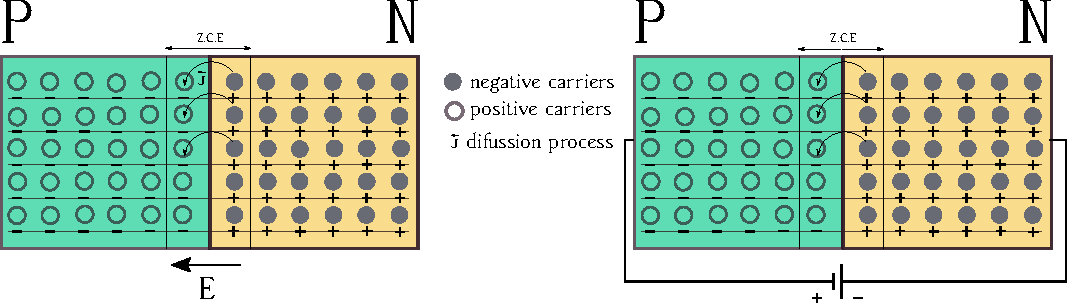
\includegraphics[width=0.6\textwidth]{figs/unionpn.pdf}
\caption{PN junction, b) PN forward bias}
\label{fig:pn}
\end{figure}

% Cuando se ha alcanzado el equilibrio, en la zona más cercana a la unión, que se conoce como \textbf{zona de carga del espacio}, los portadores minoritarios se han recombinado y en ella sólo están los iones cargados ligados a la red. El campo eléctrico originado por los iones crea una diferencia de potencial denominado, potencial termodinámico, que impide a los portadores mayoritarios pasar de un cristal a otro.

When the equilibrium is reached, the closer region to the interface called \textbf{space charge region}, the minority carriers are recombined and there are only electrically charged ions linked to the net. The electric field created by the ions generates a potential difference called, thermodinamical potential, that avoid the mjoroty carriers to cross to the other side f the juntion.

\subsection{P-N forward bias}

%Para poder hacer circular corriente a través de la unión P-N es necesario romper el equilibrio y para ello será necesario reducir el potencial termodinámico. La manera de hacerlo consiste en aplicar una diferencia de potencial entre los extremos del cristal. Si el lado P tiene una tensión positiva con respecto al lado N, la unión está polarizada en directa y en inversa en el caso contrario. Con la polarización directa, disminuye la barrera de potencialn y con ello la corriente de arrastre que ya no puede compensar la difusión. Ahora, los portadores de cada lado pueden atravesar la zona de carga del espacio y llegar al otro lado, donde son los portadores minoritarios. Ahora, el proceso de difusión provoca dos corrientes con sentidos opuestos pero de cargas diferentes, por lo que no se anulan y crean una corriente aprovechable.

If we want to make a current to cross the P-N junction it is necessary to break the balance and that means that you need to reduce the thermodinamical potential. In order to do that, we can apply a potential difference between the edges of each semicunductor. If the P side has a positive voltage with respect to the N side, the PN junction is forward bias and reverse in the other case. In the forward biases the potential barrier is reduced and then electric charge cannot compensate the diffusion. The carriers of each side can go through the charge area and reach the other side, where they are minority carriers. At this moment the diffusion process creates two currents with two opposite directions, so they do not compensate each other and it generates an usable current. 

%Cuando la unión P-N está polarizada en inversa, es decir que el lado P tiene una tensión negativa, el potencial termodinámico aumenta y no circulará ninguna corriente aprovechable.

If the P-N junction is reverse biases, which means that the P side has a negative voltage, the potential barrier increases and there will not be an usable current.

Los procesos de generación de corriente en la unión P-N pueden resumirse en la ecuación de Shockley \ref{eq:shockley} que define la corriente generada por un diodo. El diodo es el dispositivo electrónico que se basa en el funcionamiento teórico de la unión P-N. En \ref{eq:shockley} $I_0$ es la corriente de saturación del diodo en oscuridad, $V$ la tensión aplicada y $m$ un factor para ajustar al funcionamiento real y $V_T$ el potencial térmico.

The processes of current generation in the P-N junction can be summarized in the Shockley equation \ref{eq:shockley} that defines the current generated in a diode, an electronic deviced based in the P-N functioning. In \ref{eq:shockley} $I_0$  is the saturation current, $V$ the voltage applied and $m$ is a factor to adjust to real behaviour and $V_T$ is the thermodinamical potential.


\begin{equation}
  I_{D}=I_0\cdot [e^{{V}\over {m\cdot {V_{T}}}}-1]
\label{eq:shockley}
\end{equation}

\subsection{Solar Cell}

%Cuando la unión P-N es iluminada, la energía de la luz incidente puede ser absorbida por los electrones del semiconductor que pasan entonces a la banda de conducción, por el fotoeléctrico. En este proceso, se producen portadores de carga, pares electrón-hueco que son conducidos por el campo eléctrico de la unión generando una corriente. Esta corriente puede denominarse ``fotocorriente'',$I_L$, y será de sentido opuesto a la corriente del diodo.

When the P-N junction is iluminated, the incident energy can be absorbed by the electrons in the semiconductor that can jump into the conduction band, due to the photoelectric effect. Charge carriers are produced in this process because a pair electron-hole is created, this pair of carriers is then conducted due to the electric field of the junction creating a current.  

%La ecuación \ref{eq:Isolar} determina la corriente genearada por una célula solar iluminada:

The equation \ref{eq:Isolar} determine the generated current by an iluminated solar cell.

\begin{equation}
  I=I_L - I_0\cdot [e^{{V}\over {m\cdot {V_{T}}}}-1]
\label{eq:Isolar}
\end{equation}

%La fotocorriente generada dependerá en primer lugar de la energía de la luz incidente. Si su frecuencia tiene es demasiado baja, la luz no tendrá la energía suficiente para romper enlaces y atravesará el material sin ser absorbido. Por ello, no toda la luz incidente será aprovechable para generar corriente, sino que existirán pérdidas por transmisión, así como otras pérdidas por reflexión o recombinación de algunos de los portadores.

The generated phtotocurrent will depend in the first place on the energy of the incident ligth. If its frequency is not high enough, the ligth will not be able to break bonds and it will go trough the cristal without being absorbed. Due to that not all the ligth can be usable to generate current and it will exist some loses of transmission, reflection and recombination of some of the carriers.

The equivalent equation of solar cell that makes possible to model its behaviour is based on a current generator and a diode. It can be described by the next equation:

\begin{equation}
  I=I_{sc}[1-exp({\frac{V-V_{oc}+I\cdot R_s}{m\cdot V_T}})
\label{eq:Ieq}
\end{equation}

Where $I_{sc}$ is the \textit{short-circuit} current, obtain when the voltage applied to the junction is 0:

\begin{equation}
  I_{sc}=I(V=0)=I_L
\label{eq:Isc}
\end{equation}

In addition, if we apply the condition of \textit{open circuit} to the solar cell equation (I=0):

\begin{equation}
  V_{oc}=V(I=0)=m\cdot {\frac{k\cdot T_c}{e}}\cdot ln({\frac{I_L}{I_0}}+1)
\label{eq:Voc}
\end{equation}

Finally $R_s$ in \ref{eq:Ieq} represents the resistance due to semiconductor material and the metallic contacs.

% \subsection{Photovoltaic system}

\section{Links between climate and renewable energy}

%El sector energético en general y las tecnologías renovables en particular son altamente dependientes del estado de la atmósfera. La cantidad de recurso disponible en cada momento determinará, no sólo la energía final que podemos generar con las distintas tecnologías (eólica, fotovoltaica etc.), sino en muchos casos, afectará a la demanda eléctrica en situaciones meorológicas de (por ejemplo) olas de frío o extremo calor. Por ello el mercado energético y los diferentes agentes del sector, así como la necesidad de que la generación y la demanda eléctrica estén balanceadas en todo momento, necesitan de información meteorológica de alta calidad y resolución. Con ello será posible establecer y predecir la cantidad de energía que se puede generar con cada tecnología renovable. 

The energy sector in general but particularlly the renewable energy technologies are highly dependent on the state of the atmosphere. The amount of resource available at each time determine, not only the final energy that can be gnerated with different technologies, but also, it affects the electricity demand in some extreme meteorological events like heatwaves or cold spells. Due to that, energy market and different stackeholders, as well as the need of keep balance between generation and supply, demand an accurate and high resolution meteorological information. Thanks to that, it is possible to forecast the amount of energy that can be generated with each technology. 

%Por otro lado, las condiciones meteorológicas afectan de manera indirecta en otros muchos aspectos. Por ejemplo, el mantenimiento de un parque éolico offshore es un proceso extremadamente complejo debido a la accesibilidad de los aerogeneradores. Conocer de antemano la predicción meteorológica es necesario para planificar y evitar poner en riesgo a las personas implicadas.  

On the other hand, meteorological conditions affect indirectly in other aspects. For instance, the maintenance operation in an offshore wind farm is an extreme complex process due to the accesibility of the wind turbines. It is very important to know beforehand the weather forecast in order to plan the activities and avoid the risk exposure of the employees.

%Aunque las fases de operación o mantenimiento en las plantas de generación eléctrica constituyen uno de los núcleos más importantes del proyecto, es necesario considerar también algunas etapas que requieren de escalas temporales más largas. En primer lugar, para poder establecer la idoneidad de una planta de generación renovable, se establece una fase de evaluación del recurso o evaluación del potencial. En este periodo, se analizarán series temporales largas que sean representativas del recurso disponible en una zona. Esta etapa permite a los promotores establecer la energía máxima disponible que serán capaces de vender en el mercado eléctrico y será necesaria para poder establecer una financiación adecuada.

Although the short-term activities are in the core of the operational side of a renewable energy project, it is worth it to consider some stages that requires the study of longer temporal scales. Firstly, in order to establish the suitability of a renewable power plant, it is necessary to develop a resource assessment phase or potential assessment phase. This allows the owners to estimate the maximum power output of a project depending on the meteorological conditions and assess the amount of energy that they will be able to produce, what becomes important in order to finance the project.  


%En el contexto actual de calentamiento global, la relación entre energía y clima ha estado ligada habitualmente al impacto que una mayor participación de las renovables en el mix de generación puede provocar en él, considerando la posible reducción de las emisiones de gases de efecto invernadero de origen antopogénico por esta vía. Sin embargo, el hecho de que el cambio en el clima puede a su vez provocar un cambio en la disponibilidad o distribución de los recursos renovables, así como en los patrones de demanda eléctrica, debe ser investigado en profundidad. [JRC report:Climate modelling and renewable energy resource assessment].

In a global warming context, the link between energy and climate has been usually related to the impact that a big share of renewable in the generation mix can cause regarding the possible reduction of GHG in this way. However, the fact that climate change can cause at the same time variation in the availability or distribution of the resources, as well as in the electricity demand patterns, should be taken into account and thoroughly researched. 

\begin{figure}[h!]
\centering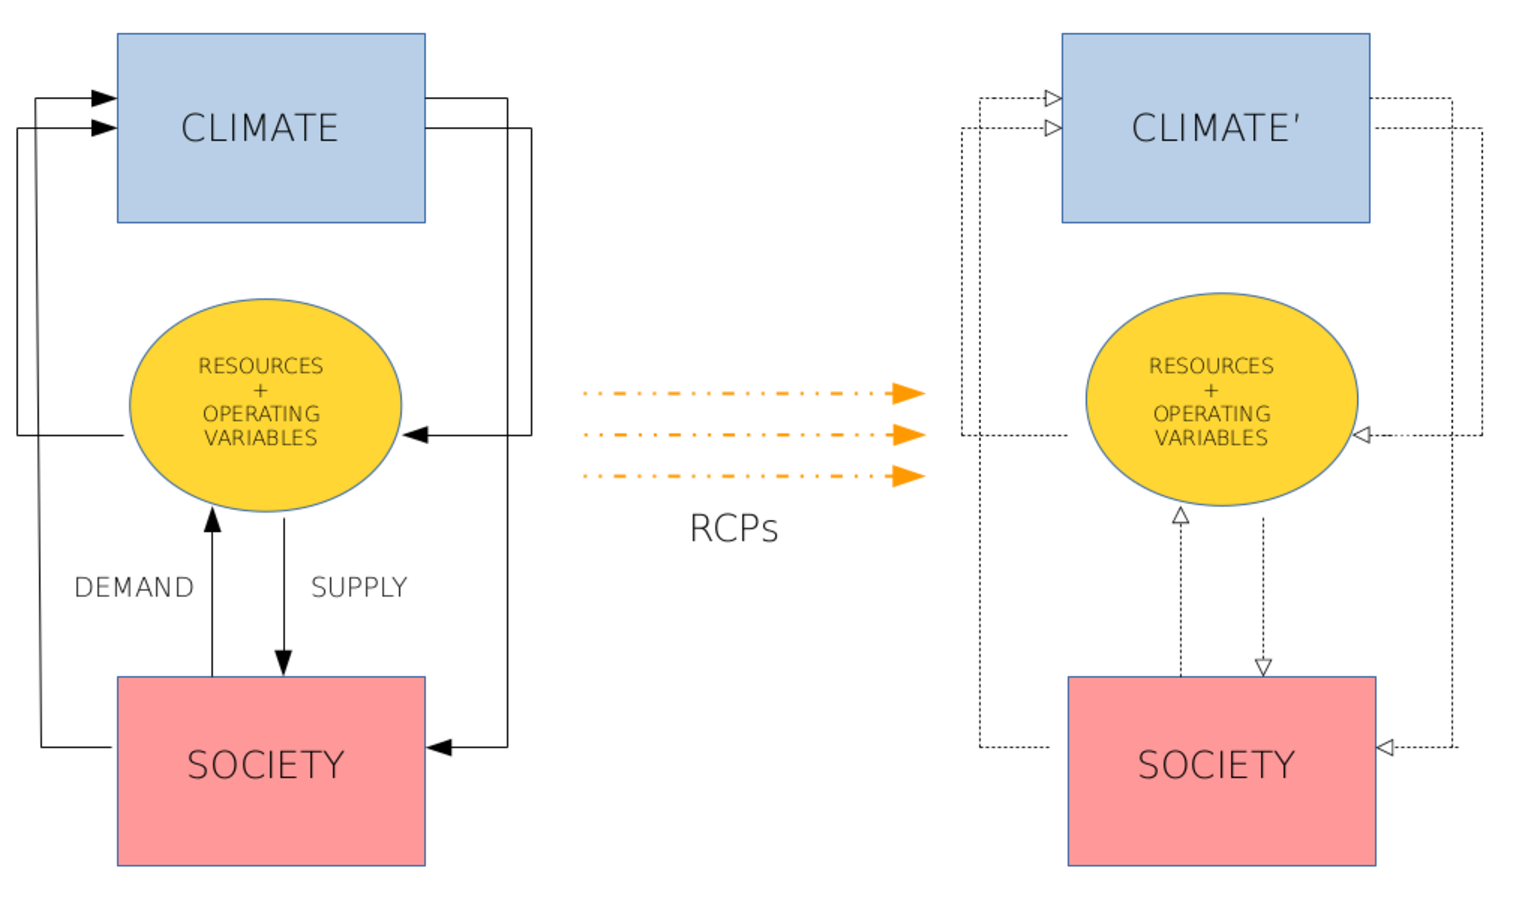
\includegraphics[width=0.6\textwidth]{figs/esquema.pdf}
\caption{Scheme: }
\label{fig:feedback}
\end{figure}

%Debido a las características intrínsecas de los recursos renovables relacionadas con su alta variablidad espacio-temporal, el sector energético demanda análisis y conocimiento profundo acerca de éstas caracteríticas en distintas escalas temporales. Esto, ayudaría a una mayor integración de las mismas así como a la mejora en la planifición, poniendo cada vez más relevancia en las escalas climáticas.

Due to the intrinsic characteristics of renewable energy resources, related to their high space-time variability, the energy sector demands analysis and deep knowdlege about that features in different time-scales. That would help to a greater integration of renewable energies as well as to an improvement in the plannification, taking more and more attention into climatic scales.

%En la figura... están representados diversos eventos meteorológicos y climatológicos que afectan a la generación energética. El eje 'x' representa las distintas escalas temporales en las que ocurren estos eventos. Es interesante destacar, aunque no es el tema principal de esta investigación, la relevancia de la escala estacional y sub-estacional para la operación de las plantas energéticas de tipo renovable. La mejora en la predicción climática en estas escalas repercutirá de forma directa en la planificación de la operación y mantenimiento, así como ayuda en la gestión por parte del operador de red y mercado. Por ejemplo, conocer con antelación si un otoño va a ser especialmente lluvioso, sirve para predecir la cantidad de electricidad que se puede producir con las centrales hidroeléctricas, haciendo el sistema mucho más eficiente y fiable. 

It is important to say, although it is out of the scope of this thesis, the relevance of the seasonal and sub-seasonal scale (and models) for the operation and maintenance of power plants. The improvement in the climate forecast on that scales will impact directly on their activities and will help to the TSO and market opeartor in the management activities. For instance, to know in advance if the next Autoumn is going to be specially rainy, will help to assess the amount of electricity the can be produced with hydropower plants, making the system more reliable and efficient.

%Uno de los problemas asociados al posible cambio en el medio-largo plazo de los recursos renovables, como puede ser el eólico, es la posible pérdida de rentabilidad de algunos proyectos que actualmente se encuentran en fase final de su vida. La repotenciación de estos proyectos con tecnologías más actualizadas, como puede ser la sustitución por turbinas eólicas de mayor potencia, junto con la prolongación de las concesiones de explotación del proyecto [ref] son una de las opciones que se dan en aquellas plantas de generación que se instalaron hace casi dos décadas. Los cambios en el recurso pueden cambiar las condiciones del proyecto no sólo por la modernización de la maquinaria y tecnología empleada, sino por el recurso disponible en la misma zona.

One of the associated problems to the possible medium to long-term changes on the renewable resources, like the wind patterns, is the possiblity of profitability loss of some projects that are now in the final stage of its lifetime. Repowering of these projects with upgraded technology, like the replace of old wind turbines by new ones with larger nameplate capacity or more efficient, is one of the options for the power plants installed almost two decades ago [ref]. Changes in the resource can change the conditions of the project not only because of the turbines used but also because of the availability of the resource.  
 
%La bancabilidad[ref] de un proyecto renovable depende de dos factores: en primer lugar su recurso y en segundo lugar, sus beneficios. Los beneficios obtenidos por el proyecto renovable dependerán del periodo de operación y de la cantidad de energía suministrada en este tiempo. Por ello, una evaluación adecuada, no sólo del recurso disponible a lo largo de todo el proyecto, sino de su variabilidad y de las posibles tendencias, es necesario a lo largo del ciclo de vida de la planta, que puede alargarse hasta 30 años[ref].

Bankabilkity [ref] of a project depends on two main factors: in first place the availability of the resource and in the second place the benefits obtained from the project. Benefits depends on the operation time and the amount of energy supplied during the lifetime of the project. Due to that, an accurate assessment, not only of the available resource, but also of its variability and trends, is necessary. 

% !! escalas climáticas: ¿es importante la repotenciacion? tener en cuenta esto? mismo recurso en el futuro?
% !! infraestructuras y extremos climáticos.

\subsection{Climate services}

%Con la creciente demanda de información por parte del sector energético de predicciones y proyecciones climáticas, aparece de manera natural la creación de los servicios climáticos para sistematizar, de alguna manera la información necesaria para los distintos stakeholders. 

With the increasing demand from the energy sector of predictions and climate projections comes naturally the climate services development, in order to systematize, to organize and to target the information for different stakeholders. [ref]

%Como puede observarse en la figure \ref{fig:feedback}, los procesos de interacción entre la sociedad y las variables involucradas en la generación de energía son de doble sentido. Por un lado el abastecimiento dependerá de la disponibilidad de los recursos y por otro, la demanda está directamente influenciada por estos factores climáticos. Teniendo en cuenta esto, el desarrollo de los servicios climáticos debe basar la mejora de sus modelos y por lo tanto, de los productos ofrecidos en estas dos premisas.

As can be seen in figure \ref{fig:feedback}, interaction processes between society and the variables involve in the energy generation are ``de doble sentido''. On one hand, the energy supply would depend on the availability of the resources and on the other hand, demand is directly influenced by those factors. Due to that, development of climate services should be base on the improvement of the models and the offered products considering the two sides.   

%La información climática en el sector energético es especialmente relevante para las descisiones estratégicas y la evaluación de riego, las operaciones de trading o la planficación de la operación y el mantenimiento en las plantas de generación (especialmente) renovables.

Climate information is specially relevant for strategic decisons, evaluation risks, planning and trading operations.

%Es relevante, aunque no es el tema de esta tesis, decir que también otros tipos de generación no renovable pueden beneficiarse de esta información y estar afectados de manera importante por algunos eventos climáticos. Por ejemplo, el aumento de temperatura del aire puede provocar una subida en la temperatura de los ríos, que ocasionalmente repercute en la operación de las plantas nucleares. En estos casos, estas plantas se ven afectadas porque no pueden continuar on las operaciones de refrigeración de los reactores (ref). 

It is relevant to say that coventional power plants can get profit of the climate services information. Some of them can easily be impacted by some extreme events like heatwaves. The above normal increase of air temperature in a heatwave episode can be related to the increase in the temperature of the river flow. That increase eventually affect the nuclear power plants operations, becasue the impacted plants are not able to use the river for their refrigeration purposes [ref].   

%\section{Resource assessment}
\section{Climate change and the Mediterranean area}

% \begin{itemize}
% \item Cambio climático de origen antropogénico a escala global. Aumento de la temperatura global.
% \item Los impactos del cambio climático ocurren en escalas locales o afectan de manera local a distintas comunidades y poblaciones de una forma desigual, relacionada también con su capacidad de adaptación y resiliencia.
% \item Por las razones mencionadas arriba, la respuesta a los diferentes impactos de cambio climático deben adoptarse de manera local, a pesar de que el consenso sobre la urgencia de actuación sea global y se adopten compromisos globales comunes.
% \item La mitigación de los grandes impactos ocurre en escala regional/local.
% \end{itemize}

%El sistema climático ha variado continuamente y de manera significativa a lo largo de la historia de la Tierra. Las variaciones del clima puede explicarse debido a factores o forzamientos externos y la respuesta del sistema climático a los mismos o, por otro lado, puede ser la causa de inestabilidades internas y relaciones no lineales entre los distintos componentes del sistema.

Climate system has varied constantly and significantly along the Earth history. Climate variability can be explained due to external factors and the response of climate system to them or on the other hand, it can be due to the internal inestabilities and non-linear relationship betwen different components of the system, the last ones occur independently of the external forcings.

%Los distintos forzamientos de origen externo pueden ser factores astronómicos, como los cambios en la intensidad de la radiación solar o en los parámetros orbitales, o bien, factores terrestres como la composición de la atmósfera debido a la actividad humana, cambios en la superficie terrestre debido al uso de la misma etc.

Different external forcings can be astronomic factors, like changes on the intensity of solar radiation or in the orbital parameters, or they can be terrestrial factors like changes in the composition of the atmosphere due to human activity, changes in the earth surface due to land use etc.

%Algunas variaciones del sistema climático ocurren de manera independiente de los forzamientos externos. Estas variaciones tienen su origen en las distintas interacciones no lineales entre los componentes del sistema climático y dan como resultado la variabilidad natural del sistema climático. 

%Some variations of the climate system happen independently of the external forcings. These variations have their origin on different no-linear interactions between different components of climate system and the result is the natural variability of the climate system.

%Desde la revolución industrial la Tierra ha experimentado un aumento de la temperatura global que no es posible explicar mediante los forzamientos externos 'naturales'  del clima como cambios en la actividad solar o en las emisiones volcánicas (Bindoff et al, 2013), ni forma parte de la variabilidad natural del sistema. El IPCC en su último informe, asegura que la actividad humana y en concreto las emisiones de efecto invernadero generadas desde la Revolución Industrial (1850) son responsables del cambio climático que ha generado el ascenso de temperatura global y que ha hecho que probablemente los 30 años entre 1983-2012 hayan sido los más cálidos en los últimos 1400 años en el hemisferio norte (IPCC). A pesar de la marcada variabilidad interanual (Stocker et al. 2013), el aumento de temperatura con caracter global en las últimas décadas es evidente. [ref de observaciones globales]

Since the Industrial Revolution the Earth has experimented an increase in the global temperature that cannot be explained due to natural external forcings like changes on solar activity or volcanic emissions (Bindoff et al, 2013), either it cannot be explained as part of the internal variability of the system. The IPCC in its last report, assure that human activity and more precisely, GHG emissions generated since 1850 are responsible of the climate change that causes the increase in global temperature and has made that probably the last 30 years between 1983-2012 have been the warmer in the last 1400 years in the northern hemisphere (IPCC). In spite of the large interannual variability (Stocker et al 2013), the global character of the temperature increase in last decades is clear.[ref de observaciones globales].

%Las consecuencias del aumento de temperatura desde un punto de vista físico dependen de la sensibilidad del sistema a los cambios en la concentración de gases de efecto invernadero. Son numerosos los estudios [ref] que se han realizado para intentar cuantificar el impacto que este aumento de temperatura puede tener en los distintos subsistemas a través de los diferentes mecanísmos de retroalimentación que pueden generarse.

%A pesar de la característica global del cambio climático, sus consecuencias e impactos son percibidos a escala local y regional. Estos impactos afectan a comunidades y poblaciones de manera desigual dependiendo de su capacidad de adaptación y resilencia. Por ello, la respuesta desde un punto de vista socio-económico para mitigar estos efectos, tiene que venir dada en esta escala, aunque exista consenso sobre la urgencia de actuación y se adopten compromisos comunes.

Despite of the fact that climate change is global concept, its consequencies and impacts are percibed in a local and regional scale. These impacts afect comunities and population unequally depending on its adaptation capabilities and resilence. Due to that, the socio-economic response to mitigate climate change impacts has to be applied in that scale although it should be a consensus on the urgency and some common compromises hava to be addopted.

%Uno de los primeros trabajos que intentaba cuantificar el impacto del cambio climático a escala local fue el de Giorgi et. al 2006. En este trabajo, se utilizaba por primera vez un índice (RCCI) para medir de forma cuantitativa y compara geográficamente las zonas más afectadas por el CC. En este aspecto, el trabajo estaba enfocado desde un punto de vista climático, es decir, el índice mide la sensibilidad del clima en esa zona. En este sentido, el Mediterráneo aparecía como una de las zonas más afectadas y desde entonces ha sido denominado como un hot-spot de CC.

One of the first works on quantification of climate change impacts in a regional scale was the one published by Giorgi et. al in 2006. They used for the first time an index, RCCI, that measured and compare geographically the climate sensitivity of different areas to climate change. The conclusion of the research showed that the Mediterranean area was the most affected area in terms of climate response to climate change, and since then it has been refered to as a climate change hot-spot.

%Los ensembles de modelos climáticos proyectan escenarios en los que las principales consecuencias del calentamiento global en el área Mediterránea son un descenso generalizado de las precipitaciones, debido a un aumento de la circulación anticiclónica asociada a un desplazamiento hacia el norte de ``Atlantic storm track''. Las temperaturas proyectadas son inusualmente altas con un ascenso especialmente alto en los meses de verano.

The climate models ensemble projects scenarios in which the main consequencies of global warming in the Mediterranean area are a generalized decrease of precipitations (with the exception of some areas like the Alps), due to an increase in the anticiclonic circulation, that is associated with a northward shift of the Atlantic storm track [ref]. Also it is projected an increase in interanual variability of temperature and precipitation, mostly in the warm season [ref]. In terms of extreme events, it is also projected less frequent but more intense precipitation events and with respect of temperature, some authors have evaluated the probability of an increase in heatwaves over the Mediterranean area [ref].   

\section{Objectives and scientific questions}%General scientific question: spatiotemporal behaviour of solar resource and photovoltaic production}

{\color{red} Hay que reescribirlo}

The main objective of this work, after being introduced the framework, is to analyse the long-term characteristics of solar resource and photovoltaic production in a relevant area, the Mediterranean region. On one hand, most of the Mediterranean region has high potential of solar resource, which makes the area suitable for its deployment. On the other hand, from the elctrical point of view, Europe is well interconnected, which is important for the development of distributed energy. In addition, due to the specially high sensitivity to climate change of the Mediterranean area and the increase in renewable energy generation it becomes an important matter.

We approach the problem in three different chapters. Each one analyses a key aspect of the long-term features of solar resource and photovoltaic production and it is made using different approaches.

% En el primer capítulo de resultados se analizará una estrategia para regionalizar una unidad geográfica con coherencia desde el punto de vista eléctrico en fucnión de sus características climáticas. En concreto se estudia la Península Ibérica por ser un sistema ``casi aislado'' de manera natural por las dificultades de interconexión con el resto del continente Europeo. 

% Por otro lado, en el capítulo 6 se estudia el papel de los aerosoles en la variabilidad del recurso y con ello en la producción. La importancia de los aerosoles en escalas climáticas y su impacto geográfico en este capítulo.

% Por último, la importancia de la proyección de los recursos renovables en las condiciones de cambio climático queda reflejada en el capítulo 7 dónde se estudia la posible evolución del recurso solar y el potencial fotovoltaico con respecto a las distintas configuraciones de aerosoles climáticos en los diferentes modelos regionales analizados.

\section{Organization of the manuscript}%\section{General scientific question: spatiotemporal variability of solar resource and photovoltaic production}

The manuscritp is organizded as follows:

The first part contains two chapters: the first one is the Introduction, that aims to overlook the context in which the thesis has been elaborated. In the second chapter it is analysed the main contributions related to the this topic over the literature. It will include the main results about intermittency of PV and how the short-term problems has been managed to go through the long-term problems. After that, the climate change perspective over the area and the main results related to solar resources are presented.

The second part includes two chapters including the Data description and the Methodology used along the studies. In this case it is important to remark that each result's chapter contains the Data and Methodology used for that specific chapter. The contents of this part are related to general description of climate data and models.

Results are presented in the third part.

Finally the fourth part contains a chapter with the main conclusions of the thesis and another chapter that summarizes the main questions emerged from the wotk, which will lead future research.

% \section{State of the art}
% \subsection{From short to long term varibility issues}
% \subsection{Solar radiation data measurements}
% \subsection{Satellite data}
% \subsection{Modelization of solar radiation}
% \section{Identification of knowdlege gaps and approach to the problem}
%\subsection{Spatiotemporal long-term variability in an almost isolated area}
%\subsection{Role of aerosols in the spatiotemporal varibility of the photovoltaic energy production}
%\subsection{Future availability of photovoltaic potential}

 
\chapter{State of knowdlege\label{cha:state}}

% \epigraphfontsize{\small\itshape}
% \epigraph{''Commençons par les systèmes les plus simples et les plus faciles à cerner pour monter graduellement à la compréhension des plus complexes.''}{--- \textup{René Descartes}, Le Discours de la Méthode}

\section{Variable renewable energies: VRE}

The variable nature of renewable energy resources, in space and time, is a key aspect for their high penetration into the conventional electicity systems. Due to the fact that supply and demand have to match at every time-step, the forecast and management of the electricity produced with 'variable renewable energy (VRE)' plants is necessary to acomplish this match. In the traditional electricity systems, a portfolio of centralized power plants (coal, nuclear, gas...) dispatch electricity as customer loads demanded it. The conventional power plants are able to storage the primary energy that they use and only produce electricity when it is needed. With the increase of wind and solar power plants, the supply of electricity demand approach has changed. The VRE power plants only produce electricity when enough resoruce is available and in the case of photovoltaic power plants, only during the daylight time. This concept has being refered as \textbf{intermittency}, to recall the fact that solar and wind resources are not available at any time and that they are variable in different time-scales. Because of the fact that electricity cannot be storage, they are non-dispachable power plants and the operation of the system has to be addapted. However, the alternatives of energy storage from VRE plants are increasing in different ways: batteries for wind and photovoltaic power plants, hydrogen or pumping hydropower \cite*{Lund2015, Blanco2018, Schaber2004}.

The research in storage for VRE is rising but different approaches are also being addopted to integrate high share of this alternative technologies. The term \textbf{flexibility} is one of the most used refered to the new strategies followed from the demand and supply side in order to adapt to the new system \cite*{KROPOSKI2017}. From the demand side, flexibility refers to means related to load shape and demand patterns, like peak saving, load shifting, valley filling etc \cite*{Lund2015}.

On the other hand, flexibility of the supply side depends on the power plants, whose output can be controled to obtain power balance. It is important in terms of flexibility to consider the response time of different power plants as well as the different nature of each one. As the availability of solar and wind resources are not related to the geographical distribution of the demand, a highly interconnected grid is one of the main needs for high VRE penetration. Once this is considered, geographycally spread portfolio of VRE plants are able to smooth variability of power output \cite*{KROPOSKI2017, Marcos2012}(Hoff and Perez 2012, 2013, añadir más referencias).

%* Explicar más el concepto de smoothing?? agregar aquí todas las citas de smoothing

There are also studies that try to identify complementarity features of different energy resources either in time or in space in order to address the intermittency issue through the smooth of the power output. The complementarity studies are made using different technologies like hydropower and wind power \cite*{Denault2009, Silva2016} or hydropower and solar photovoltaic \cite*{Francois2016, Beluco2012, Kougias2016}. In \cite*{Hoicka2011} complementarity of wind and solar is investigated for a region in Canada and in \cite*{Monforti2014} local complementarity is investigated in Italy.

%** Incluir las citas de Sonia?? 

As much as we were able to predict/forecast the variability of solar/wind resources, better flexibility measures and strategies could be apply to integrate high rates of VRE without compromise reliable and efficiency. 
% For example on the supply side, the kind of flexibility is accomplished through power plants with
% different response time. Introducing variable power generation such as wind and solar power may
% increase the need of energy system flexibility, which could be accomplished through additional measures
% on the supply or/and demand side which is the subject of this paper. From the electricity system point of
% view, flexibility relates closely to grid frequency and voltage control, delivery uncertainty and variability
% and power ramping rates
\section{Variability sources in PV}

It is important to notice that every power system has associated an inherent uncertainty and variability and it is not only a renewable energy systems characteristic. In the case of PV systems, the variability of PV outputs depends on the variability linked to the solar irradiation reaching the generator (resource variability), and also depends on the behaviour of the electrical components.  

% ``Before focusing on the variability and uncertainty of PV plants, it is important to understand that
% variability and uncertainty are inherent characteristics of power systems. Loads, power lines,
% and generator availability and performance all have a degree of variability and uncertainty
% It is clear that uncertainty in photovoltaic power it is a combination of the uncertainty of estimation of solar resource and the uncertainty in the behaviour of the electrical componentes of the photovoltaic system.''

\subsubsection{Astronomical factors}

The amount of solar energy that reach the photovoltaic generator depends on the first place on the sun position, which is a deterministic factor that only depends on the time of the year and the day-time. It means that the first factor causing PV intermittency is the fact that no energy can be produced during nigth-time. However, although this daily scale intermittency is the one that most affects the PV power production there is no uncertainty associated to this fact, which is a very important concept in order to manage VRE.

\subsubsection{Clouds}

There are other factors that affect the solar energy reaching the surface and it depends on the composition of the atmosphere at each time. When solar radiation goes through the atmosphere it can be reflected, absorbed or scattered. The presence of clouds is the most affecting factor in the transmission of solar radiation to the surface. The condensed particles that forms clouds makes solar radiation being scattered and reflected and part of the radiation can also be absorbed. Different types of clouds affects differently to solar radiation. High thin clouds are less dense than low clouds, becoming more transparent to solar radiation. Also, some clouds are less spatially aggregated than others. When the sky is overcasted, the amount of energy reaching the surface decrease but the frequency of the intermittency generated in the PV output is not as high as if some individual clouds pass through.

The time scales affected because of clouds varies from seconds to minutes. The intermittency due to clouds is very high as well as its uncertainty, because the exact position of clouds is sometime very difficult to forecast.

\subsubsection{Aerosols}

In the absence of clouds, aerosols \footnote{Aerosols is the term used to refered to the solid particles suspended on gas. In this wotk we are referin g to the atmospheric aerosols, which are the solid particles suspended on the atmosphere but the hydrometheors like ice crystals} are the main source of variability for solar resource. 

Aerosols impact solar radiation in two ways: directly, scattering, absorbing or reflecting solar radiation or indirectly, acting as condensation nuclei favouring the formation of clouds [ref].

Time scales involved varies from daily to seasonally, because in some places the presence of aerosols have a very strong seasonality. Also, due to the highly related influence of aerosols and human activities (depending on the aerosols type), it has been detected that in longer time scales solar resource is also affected by changes in aerosol content.

%Gueymard, C.A. Temporal variability in direct and global irradiance at various time scales as affected by
%aerosols. Solar Energy 2012, 86, 3544 – 3553.

\subsubsection{Other factors}

As it has been noted at the beginning of the section, there are othter factors that affects the performance of the PV system, causing variations in the PV output. These factors are related to the electrical components of the system and they can be divided into internal and external facors.

The most important external factor affecting the performance of the system is temperature. It affects cells performance and if temperature is highly different than the optimun cell temperature the efficiency will drop. Also some external factors like dust deposition can affect the electrical performance, limiting the energy reaching the cell.

Internal factors affecting the PV output that can cause variability are related to the transmission lines, wires and interconnections, or the inversor.

\section{Photovolatic power forecasting}

The energy obtain from a photovoltaic system can be estimated if the amount of solar energy that reach the generator surface is accurately predicted. The prediction of solar irradiation variability enhance the forecast of the energy output. Solar radiation varies across multiple time-scales, from seconds to multi-decadal variations. To understand those changes helps different stages of the project and electricity generation.

There are different types of forecasting methods for solar power, they are based on the models that forecast solar irradiation. Among them there are two different approaches: \textbf{physical methods} and \textbf{statistical methods}. Physical methods are based on the radiative transfer equation and physic variables whereas the statistical or empirical methods are based on historical fata. Some approaches are also \textbf{hybrid} approaches that combined both \cite*{Diagne2013, Tovar-Pescador2008}. They mainly rely on two principles: first an estimation of the clear-sky irradiance and secondly, they account for the presence of clouds [ref Jan Kleiss].  


\subsection{Solar irradiation forecasting}

The application of each kind of the forecasting models is very related to the forecast horizon that want to be addressed as well as the horizontal resolution. We refers here to the short-term issues in photovolaic power forecasing: in the operation activities, 3 time forecasting horizons were described by Kostylev and Palovsky \cite*{kostylev2011solar}: intra-hour, intra-day, day-ahead. For trading purpose, the day-ahead forecast is very important and for planning operations in longer time-scales seasonal forecast will be a very valuable asset if model skill improves [ref]. 

\subsubsection{Physical Methods}

The physical modeling of solar radiation is based on physical equations of the interaction between atmospheric components and solar radiation (aerosols, water vapour, clouds...). When solar radiation goes through the atmosphere, it can interact with its components being absorbed by molecules, backscattered to space or scattered in any other direction. Thus, only part of the solar radiation at the top of the atmosphere (TOA) will reach the Earth's surface.

This process is the physical process of energy transfer described by the radiative transfer equation (RTE) and its solution needs a radiative transfer model (RTM). The radiative transfer is a very complex process that needs to be simplified to be solved numerically and some parametrizations are needed. However, from these models it is possible to reproduce the solar radiation behaviour across the atmosphere and at the surface. RTMs are in the core of numerical weather prediction models, NWP, and climate models and sometimes they are used to obtain solar radiation from satellite images, although in this case empirical or semi-empirical approaches are also commonly applied.

Numerical weather prediction models are very useful in a time range from 4h to 6h and they are also applied for the day-ahead forecast. It is very frequent to apply a post-processing process to the output of NWP that enhance the forecast. Some statistical tools like bias correction can be apply to reduce some systematic errors or local effects \cite*{Diagne2013}.

\subsubsection{Statistical methods}

Solar radiation at the surface can be estimated also using statistical methods. In this case it is necessary to have enough historical data to create and validate the model and likely these models will not be able to reproduce solar behaviour universally. However, they can be very useful for local applications and at very high time-resolution.

Under these methods tradicionally used to forecast time-series, relies the idea of predict some variables trought the statistical analysis of historical data and its relationship with other variables called predictors. Many models have been developed in this sense from the most simple approach, the persistence model, or autorregressive models to more sofisticated ones \cite*{Reikard2009, bacher2009, Inman2013}. 

Developing of the ANN and non-linear models have been also applied to solar forecasting field, in that case the predictions are based on an algorithm learning \cite{Mellit2008}. 


% Statistical methods have been used successfully in time series forecasting for
% several decades. Using the statistical approach, relations between predictors,
% variables used as an input to the statistical model, and the variable to be predicted,
% are derived from statistical analysis. Several studies with respect to
% direct time series modeling have been performed. In Reikard [2], different time
% series models are compared. In Bacher and al.[7], the authors investigate the
% use of a simpler AR model to directly predict PV power in comparison with
% other models.
\subsubsection{Hybrid methods}

It is very common to apply a combination of more than one model to enhance the prediction accuracy. Many studies have shown the overcome of a combination of two different approaches with respect to a simpler approach \cite*{Diagne2017, Yang2014}. For instance, some studies show the aplication of ANN methods after the obtention of NWP output \cite*{Cornaro2015} or after obtain a satellite-based model output \cite*{Marquez2013}\\ 

\begin{figure}[h!]
\centering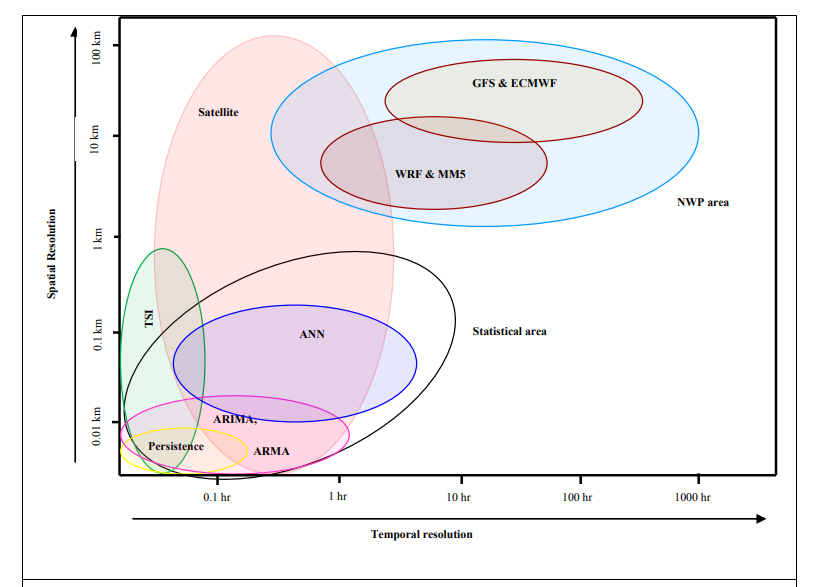
\includegraphics[width=0.6\textwidth]{figs/forecast.png}
\caption{Models to forecast irradiance depending on the time horizon. Incluir ref aunque se va a rehacer}
\label{fig:forecast}
\end{figure}


Different models are applied depending on the forecast horizon as they are summarized in the figure. Usually, the main steps in the solar irradiation forecast are first the estimation of the clear-sky irradiance and after that account for the presence of clouds ref[Jan Kleiss].


% incorporates two or more techniques and produces a new
% forecasting method with improved accuracy. In this method
% the deficiencies of the individual model are overcome and
% advantages of individual models are utilized. These methods
% also reduce the forecast errors. For evaluating the forecast
% errors solar forecasting evaluation metrics are also studied.
% Forecasting evaluation metrics allow to understand how much
% to trust the forecast and re-evaluate it in case of high errors.

\subsection{Clear-sky models}

Among the different approaches to model or forecast solar irradiation at the surface clear-sky models deserves special attention. These models estimate solar irradiation under clear-sky conditions, which means that the attenuation of solar irradiation is only due to the consitituents of the atmosphere and not due to clouds.

The difference between clear-sky models is based on the parameters used to predict solar irradiance. The most simplest ones only consider the zenith angle and extraterrestrial irradiation. The higher the complexity of the model, the more parameters are included to characterize the state of the atmosphere: different aerosols content, water vapour etc. 
The amount of energy that reaches the surface depends on the transmittance of the atmosphere. The incident extraterrestrial irradiance at the top of the atmosphere (TOA) would be attenuated depending on the composition of the atmosphere thus in the air mass (AM) crossed to reach the surface. For the latter reason, the zentih angle is the first factor to consider when the surface solar irradiation want to be estimated: with higher zenith angles, higher the air mass. The simplest models based on this parameters are empirical relationships based on measurements for an specific location. Evaluations of these models have shown that it is necessary to take care when applying for a different location that the one used for its calibration \cite*{Badescu1997, Davies1989}.

In addition to these simple models, some parameters can be considered enhanzing the performance of the forecast. The Kasten model [] and the Inchen and Perez [] (that is a modification of the first one) use the zenith angle, the air mass, the elevation and the the Linke turbidity, a parameter that describes the optical thickness of the armosphere.

The most sophisticated clear-sky models includes more parameters like the ozone, aerosols and precipitable water. Some of the most used models are Bird, MAC, or REST2[]. There are several studies that summrizes a benchmark of different clear-sky models \cite*{Gueymard2013a,b}. It is clear that there is a relationship between the more atmospheric variables included in the model, the better the performance. But measures of all variables included are not always available. Due to that reason, the best model would arise from a balance relationship between the availability of atmospheric measurements to calibrate the model and its performance. 
 
% Referencia para esta clasifion: Global Horizontal Irradiance Clear Sky Models: Implementation and Analysis

\subsection{Satellite-based models}

Due to the scarcity of solar radiation measurements, the availability of satellite data has become an important trigger for the development of targetted products for the solar industry [ref].

There are different methods to retrieve solar radiation from satellite images that goes from physical models to empirical ones. In the first case, the models try to explain the radiance observed by the satellite instrumentation with a radiation transfer model (RTM). In order to do that, it is necessary to know the composition of the atmosphere. On the other hand, empirical models are based on simple regression models between the visible-channel's recorded intensity and grounded measurements. 

It is possible to extract cloudiness information from the satellite radiance information due to the fact that intensity of the measurements change depending on the composition of the atmosphere and the cloud cover. Considering that, a simple equation can describe the relationship between the radiance measured and the amount of clouds, this was called \textbf{cloud index [Cano].}

To retrieve solar radiation form satellites, most empirical methods considers a linear relationship between the cloud index and atmospheric transmittance \cite*{Polo2008} [Polo libro, (Cano et al. 1986; Diabaté et al. 1988; Schmetz. 1989; Diabaté et al. 1989; Noia et al. 1993a; Ineichen and Perez. 1999; Zelenka et al. 1999; Perez 2002; Rigollier et al. 2004; Zarzalejo et al. 2005)].  

%* cloud index?
%* clear sky index ?

There are also some approaches that are in between theses two sides: the semi-empirical models, which have become the most common approach \cite*{Polo2008}. They use a simple radiative-transfer scheme and some statistical regressions between data from satellite sensors and observed data (Schmetz (1989), Noia et al. (1993), Pinker et al. (1995), Zelenka (2001), and Hammer et al (2003)).\footnote{Jan Kleiss, Solar Energy Forecasting and Resource assessment, pp.22.23}

% The importance of the cloud index concept bases on the fact that satellite
% information (basically cloud cover information) can be related with the solar irradi-
% ance incoming to the earth surface. Consequently, most empirical/statistical method-
% ologies to retrieve solar irradiance from satellite images rely on the assumption
% of linear relationship between the atmospheric transmittance and the cloud index
% (Cano et al. 1986; Diabaté et al. 1988; Schmetz. 1989; Diabaté et al. 1989; Noia
% et al. 1993a; Ineichen and Perez. 1999; Zelenka et al. 1999; Perez 2002; Rigollier
% et al. 2004; Zarzalejo et al. 2005).


There are two types of satellites orbiting the earth: The polar orbiting, closer to the earth surface,  with high spatial resolution but limitations in the temporal coverage, and the geostationary satellites (~36000km from the earth's surface) with high spatial and temporal resolution. This last kind of satellites are the commonly used to derived solar radiation at the surface.

The uncertainty in the satellite radiation estimation comes from different sources. First, Sun elevation affects the determination of clouds position due to the increase of reflections, increasing  the uncertainty for low Sun elevation. Other factors are related to geographical factors. The high albedo of some surfaces like desserts or ice areas makes difficult the determination of clouds, increasing uncertainty (Cebecauer et al. 2011).


% Physical methods are those based on atmospheric data such as temperature, pressure
% The physical method is based on the numerical weather
% prediction (NWP), cloud observations by satellite or Total Sky
% Imager (TSI) or atmosphere by using physical data such as
% temperature, pressure, humidity and cloud cover.

% Nowadays, the most used method is the hybrid method which
% incorporates two or more techniques and produces a new
% forecasting method with improved accuracy. In this method
% the deficiencies of the individual model are overcome and
% advantages of individual models are utilized. These methods
% also reduce the forecast errors. For evaluating the forecast
% errors solar forecasting evaluation metrics are also studied.
% Forecasting evaluation metrics allow to understand how much
% to trust the forecast and re-evaluate it in case of high errors.
% \subsection{Physical methods}

% \subsection{Statistical methods}
% \subsection{Hybrid methods}

% ``For non-concentrating systems (such as most PV systems),
% primarily the global irradiance (GI = diffuse + DNI) on a tilted
% surface is required which is less sensitive to errors in DNI
% since a reduction in clear sky DNI usually results in an
% increase in the diffuse irradiance. Power output of PV systems
% is primarily a function of GHI. For higher accuracy, forecast
% of PV panel temperature are needed to account for the (weak)
% dependence of solar conversion efficiency on PV panel
% temperature.''

\section{From short to long term issues}

Longer time scales has been evaluated for other stages of PV projects like resource assessment. This phase consist on the evaluation of solar resource in order to estimate the potential energy that can be obtain with a project in an area. Also, this estmiation is been useful for communticating potential of different renewable energy resources across different countries to plan and define strategies by policymakers.

Solar \textbf{resource assessment} needs long time series of solar irradiation data in order to capture the climatic characteristics. In that sense, it would be necessary a wide-spread network of stations recording solar radiation. Up to now, the scarcity of this measurements makes difficult to obtain accurate and long time series for every place where the solar resource wants to be measured. Satellite data has become the best option to get long time series record of high spatial and temporal resolution data. These data allows to characterize variability which is useful to determine the suitability of a short-term data set to produce valid long-term statistics [NREL, best practices]. For instance, it is common to use a typical meteorological year to assess the potential energy in a place. However, some studies has shown that this practice it is not accurate, at least for certain places, if direct normal irradiation (DNI) want to be characterize [Gueymard]. Years with higher loads of aerosols, which affects directly on DNI, are excluded if only TMY is used for the financial assessment of a CSP proyect. Global solar irradiation is less variable than direct normal irradiation, but quantifying inter-annual variability becomes important in all solar projects favouring management.

%* seasonal ?? Interannual Variability and Seasonal Predictability of
%Wind and Solar Resources

Variability of solar resources in monthly to seasonal time scales has been evaluated related to large-scales circulation modes [Interannual Variability and Seasonal Predictability of Wind and Solar Resources, S.Jerez]. Certain grade of correlation between solar (and wind) anomalies and these modes has been found [ref]. To the extent that those modes are predictable they could be directly linked with anomalies in solar (and wind) resource, which would help in the seasonal forecasting for solar power, although these correlations greater for some locations rather than a global behaviour. Some results has been seen in these sense for wind seasonal forecasting and its relationship with the NAO [Clark, R.T.; Bett, P.E.; Thornton, H.E.; Scaife, A.A. Skilful seasonal predictions for the European energy industry. Environmental Research Letters 2017, 12, 024002]


% Some of this variability
% correlates with values of climate modes, and persistence and predictability of these modes provides
% the potential for skill in seasonal prediction of these wind and solar fluctuations

% Both wind and solar monthly anomalies were found to show some correlation with the climate
% modes tested. To the extent that these climate modes are persistent or dynamically predictable,
% long-range forecasts of these anomalies are possible. Statistical and dynamical methods can be used
% to predict sea surface temperatures [30,57,58], which are strongly associated with many of the climate
% modes, and there are also other sources of seasonal predictability, for example related to snow cover
% and soil moisture [59,60]. Thus, improvements in NAO forecasting have led to better winter wind
% power forecasts over Europe [61].
% Many of the teleconnection correlations, particularly those for AO and NAO in winter (Figures
% 5 and 6), are of opposite sign between northern and southern Europe, implying that spreading and
% interconnecting wind and solar generation across the continent can mitigate the impact of interannual
% variability on power supply. Similarly, positive correlations between wind and solar variability, such
% as that seen in the southwestern US, can suggest the need for additional provision for reserve power
% or grid interconnections.
% Predictability based on these climate modes is seen to be much greater for some locations and
% seasons than is the case in the global mean. The climate modes used here, taken from NOAA, are
% ones that are known to influence weather in the United States. For other locations, for example in
% the Southern Hemisphere, other climate modes, such as the Antarctic Oscillation [62], could have
% stronger associations with wind and solar fluctuations.


In longer perspectives, trends have been also evaluated because of multi-year variability and the presence of periods known as “dimming” and “brightening” (Müller et al. 2014, Wild 2015). Several studies have shown that those periods had occured in different areas in last decades. The \textbf{dimming} period over Europe over the 80's and its following \textbf{brigthening} period has been extensively evaluated [ref] and it has been proved that anthropogenic aerosols over the area are responsible of the former and its decrease of the latter.[ref]
 
%``Long-term trends in GHI and DNI are also of importance because of the succession of periods known as “dimming” and “brightening,” which affect both climate change and the extrapolation of the historical solar resource into the future (Müller et al. 2014, Wild 2015)''

%* papers de resource assessment
%* typical meteorological year y sus problemas con los aerosoles y CSP? 

%However, solar radiation is the most relevant variable in the energy balance of the Earth, wich means that its study is itself important for the complete understanding of the climatic system. There are many studies focused on solar radiation variabilitity at the surface that try to understand low frequency changes, observed trends and interanual variability of solar resource over Europe.

%* Interanual variability
%* decadal/multidecadal changes


{\color{red}I have doubts about continue this section with all the results about solar radiation studies in Europe}

\section{Climate Change perspectives for solar resource and photovoltaic potential}

%* Explicar aquí que se hace un cambio de perspectiva utilizando modleos climáticos¿?

%``Long-term trends in GHI and DNI are also of importance because of the succession of periods known as “dimming” and “brightening,” which affect both climate change and the extrapolation of the historical solar resource into the future (Müller et al. 2014, Wild 2015)''

In a context of climate change, the climate system will evolve and renewable energy resources can be affected. Some studies had started to evaluate this resources under different climate change scenarios. The first technology that can be impacted is hydropower, due to the fact that many studies had showed that for mid-lartitudes precipitation will decresase and with respect to extreme events, drougth could become more frequent [].

Some studies for Europe shows a sligth decrease of wind potential for southern Europe, with an increase in the nothern areas [].

Solar radiation potential under climate change scenarios has been investigated in several works: Crook, Wild, Jerez, Tobin and Bartok. Some of theme are focused on solar radiation (Bartok) rather than in photovoltaic potential beause they have a climate perspective. Global projections has been evaluated in [][] showing an increase in some areas like Europe, East-Asia and . An slightly decrease is also shown by [] over .

Other works shows regional results, focused on a region. Main results in solar resource shows a discrepancy between Global Models, GCMs, and Regional Climate Models, RCMs\footnote{Climate models are explained in section x of chapter 4}, over Europe.

The discrepancy showed by GCMs ans RCMs is the main issue followed to analyse in chapter 7 which are the reasons for it.

%\end{document} 